% Created 2022-04-24 Sun 20:11
% Intended LaTeX compiler: pdflatex
\documentclass[titlepage,a4paper]{article}
\usepackage[utf8]{inputenc}
\usepackage[T1]{fontenc}
\usepackage{graphicx}
\usepackage{longtable}
\usepackage{wrapfig}
\usepackage{rotating}
\usepackage[normalem]{ulem}
\usepackage{amsmath}
\usepackage{amssymb}
\usepackage{capt-of}
\usepackage{hyperref}
\usepackage{minted}
\usepackage{a4wide}
\usepackage[colorlinks=true,linkcolor=black,urlcolor=blue,bookmarksopen=true]{hyperref}
\usepackage{bookmark}
\usepackage{fancyhdr}
\usepackage[spanish]{babel}
\usepackage[utf8]{inputenc}
\usepackage[T1]{fontenc}
\usepackage{graphicx}
\usepackage{float}
\usepackage{minted}
\usepackage{svg}
\pagestyle{fancy}
\fancyhf{}
\fancyhead[L]{TP2 - Grupo 1}
\fancyhead[R]{Teoria de Algoritmos I - FIUBA}
\renewcommand{\headrulewidth}{0.4pt}
\fancyfoot[C]{\thepage}
\renewcommand{\footrulewidth}{0.4pt}
\usemintedstyle{stata-light}
\newminted{c}{bgcolor={rgb}{0.95,0.95,0.95}}
\usepackage{color}
\usepackage[utf8]{inputenc}
\usepackage{fancyvrb}
\usepackage[usenames,dvipsnames]{xcolor}
\fvset{framesep=1mm,fontfamily=courier,fontsize=\scriptsize,numbers=left,framerule=.3mm,numbersep=1mm,commandchars=\\\{\}}
\author{Pablo Andres Dealbera}
\date{\today}
\title{}
\begin{document}

\begin{titlepage}
	\hfill
\includegraphics[width=6cm]{assets/logofiuba.jpg}
    \centering
    \vfill
    \Huge \textbf{Trabajo Práctico 2 — Algoritmos D\&C y Programacion Dinamica}
    \vskip2cm
    \Large [75.29/95.06] Teoria de Algoritmos I\\
    Primer cuatrimestre de 2022\\
    \vfill
    \begin{tabular}{ | l | l | l | }
      \hline
      Alumno & Padron & Email \\ \hline
      BENITO, Agustin & 108100 & abenito@fi.uba.ar \\ \hline
      BLÁZQUEZ, Sebastián & 99673 & sblazquez@fi.uba.ar \\ \hline
      DEALBERA, Pablo Andres & 106585 & pdealbera@fi.uba.ar \\ \hline
      DUARTE, Luciano & 105604 & lduarte@fi.uba.ar \\ \hline
      PICCO, Martín & 99289 & mpicco@fi.uba.ar \\ \hline
  	\end{tabular}
    \vfill
    \begin{tabular}{ | l | l | }
      \hline
      Entrega: & Primera \\ \hline
      Fecha: & Miercoles 27 de Abril del 2022 \\ \hline
  	\end{tabular}
    \vfill
    \vfill
\end{titlepage}
\tableofcontents
\newpage
\definecolor{bg}{rgb}{0.95,0.95,0.95}

\section{Parte 1: Un evento exclusivo}
\label{sec:org35823f3}

Para esta primera sección, se plantea un problema en el que, dado un ranking 
de jugadores que corresponde a este año, y la posición de cada jugador en el 
ranking del año anterior, hallar para cada jugador la cantidad de jugadores
que superó en el ranking de un año a otro (i.e. con cuántos se invirtió el
órden relativo)

\subsection{Resolución por Fuerza Bruta}
\label{sec:orgbb2dcca}

Para cada uno de los jugadores en el ranking actual se evalúan los siguientes hasta el final del ranking. En dicha iteración se aumenta un contador cada vez que se encuentre un jugador con un ranking menor al del año pasado que el jugador que se está recorriendo actualmente. Por último, se guarda dicho contador en una lista y al finalizar las iteraciones se devuelve dicha lista.

\subsubsection{Pseudocódigo}
\label{sec:org619a882}

\begin{minted}[bgcolor=bg]{text}
def rivales_superados(listado):
    resultados = lista_de_igual_longitud_que(listado)
    for jugador, indice in listado:
        resultados[indice] = 0
        for rival, _ in listado.slice(indice + 1):
            if jugador.ranking_anterior > rival.ranking_anterior:
                resultados[indice] += 1
    return resultados
\end{minted}

\subsubsection{Complejidad temporal}
\label{sec:orgf1cdc4e}

Por cada jugador se recorren todos los siguientes, lo cual conlleva a una complejidad de \(O(n^2)\).

\subsubsection{Complejidad espacial}
\label{sec:orgfd2c5b1}

Los resultados a devolver ocupan \(O(n)\) y el resto de las variables son constantes, consecuentemente la complejidad espacial es \(O(n)\).

\subsection{Resolución por División y Conquista}
\label{sec:orgffde9df}

\subsubsection{Idea General}
\label{sec:orgc52a29d}

La resolución planteada por división y conquista es similar al ejercicio “Contando inversiones”. En este caso la idea es partir del listado ordenado por el ranking actual, dividir el problema por la mitad de forma recursiva y luego desenrrollar la recursividad ordenando por el ranking del año pasado. Al realizar este proceso veremos los rankings que “se cruzan” lo cual permitirá aumentar el contador de los rivales superados.

Como el objetivo es obtener esta cantidad en forma individual para cada jugador, haremos uso de un diccionario o lista para almacenar la información. Además, debe realizarse una ligera modificación del algoritmo para poder adaptarse a este requerimiento. La versión original se enfoca en contar la cantidad total de inversiones, lo que logra a través de acumular durante la etapa de merge los “elementos restantes por insertar” en el arreglo inferior al momento de insertar un elemento del arreglo superior (si estamos insertando uno del superior, quiere decir que todos los otros restantes del arreglo inferior deberían ir después que este, por lo que están invertidos); sin embargo, el algoritmo no discierne con cuántos otros un elemento está invertido.

Por ejemplo, siguiendo el ejemplo dado en la consigna, siguiendo la ejecución se llega al merge de los arreglos [(E, 6), (D, 8)] y [(F, 5)]. El algoritmo comienza a unificarlos, pero al notar que es el elemento del segundo arreglo el de menor valor, contará todos los elementos del primer arreglo por insertar (en este caso 2) como inversiones. Sin embargo, no distingue que hubo una inversión (E, F) y otra (D, F).

Para solventarlo, la modificación es sencilla: realizar el merge en sentido inverso, en orden descendente en lugar de ascendente, comenzando a unir por el final de cada arreglo en lugar del comienzo. Para el mismo ejemplo: primero comparamos D con F, como D es mayor, lo insertamos en el arreglo mezcla y, como esperábamos que fuese menor, contamos una inversión para D; continuando, comparamos E y F, y volvemos a estar frente al mismo caso; luego, solo queda insertar F. De esta manera, se siguen contando 2 inversiones, pero ahora se distingue con quiénes se dió cada una. Dependiendo de la implementación, el arreglo puede construirse insertando siempre al principio, de manera que quede ascendente, o construirlo descendente y luego invertirlo.

\subsubsection{Pseudocódigo}
\label{sec:orge29a7c1}

\begin{minted}[bgcolor=bg]{text}
funcion rivales_superados(jugadores)
    sea superados un diccionario
    rivales_superados_rec(jugadores, superados)
    devolver superados

funcion rivales_superados(lista, superados)
    si | lista | <= 1:
        devolver lista

    dividir la lista en dos mitades: lista_inf, y lista_sup

    lista_inf_res = rivales_superados_rec(lista_inf, superados)
    lista_sup_res = rivales_superados_rec(lista_sup, superados)

    lista_final = unir_y_contar_superados(lista_inf, lista_sup, superados)

    devolver lista_final

funcion unir_y_contar_superados(lista_inf, lista_sup, superados)
    sean los índices i = |lista_inf|, j = |lista_sup|
    sea resultado una lista vacía de largo i + j - 1
    
    mientras 0 <= i y 0 <= j:
        sea a = lista_inf[i]
        sea b = lista_sup[j]
        si lista_sup[j].ranking < lista_inf[i].ranking:
            resultado[i+j] = a
            superados[a] += 1
            i--
        si no
            resultado[i+j] = b
            j--

    mientras 0 <= i:
        resultado[i+j] = lista_inf[i]

    mientras 0 <= j:
        resultado[i+j] = lista_sup[j]

    devolver resultado
\end{minted}

\subsubsection{Complejidad temporal por Teorema Maestro}
\label{sec:orge8e0d40}

El teorema del maestro establece que, dados \(a\) y \(b\) constantes, \(f(n)\) una función, \(T(n) = a * T(n/b) + f(n)\) una recurrencia con T(0)=cte:
\begin{itemize}
\item Si \(f(n) = O(n^{log_b a - e}), e > 0 \Rightarrow T(n) = \Theta(n^{log_b a})\)
\item Si \(f(n) = \Theta(n^{log_b a}) \Rightarrow T(n) = \Theta(n^{log_b a} * log n)\)
\item Si \(f(n) = \Omega(n^{log_b a + e}), e > 0 \Rightarrow T(n) = \Theta(f(n))\)
\end{itemize}

Para el caso, podemos establecer que \(T(n) = 2 T(n/2) + O(n)\), dado que el problema se divide en dos subproblemas de \(n/2\) elementos cada uno (contar inversiones en dos mitades de una lista) y, adicionalmente a los dos subproblemas, se realiza una iteración de los resultados para unir y ordenar las listas en una única, contando las inversiones en el proceso, lo que supone \(O(n)\) por iterarse \(n/2+n/2\) elementos.

De la relación de recurrencia observamos que \(a=b=2\). Analizando caso a caso:
\begin{itemize}
\item \(n^{log_2 2 - e} = n^{1 - e}\). Como \(e > 0\), no se puede satisfacer que \(f(n) = n = O(n^{1-e})\), dado que \(n^{1-e} \leq n, \forall n > 0\), por lo que el caso queda descartado
\item \(n^{log_2 2} = n\). Se satisface que \(f(n) = n = O(n)\)
\item \(n^{log_2 2 + e} = n^{1 + e}\). Como \(e > 0\), no se puede satisfacer que \(f(n) = n = \Omega(n^{1+e})\), dado que \(n^{1+e} \geq n, \forall n > 0\), por lo que el caso queda descartado
\end{itemize}

En conclusión, por teorema maestro, la complejidad temporal es \(T(n) = \Theta(n^{log_2 2} * log n) = \Theta(n log(n))\)

\subsubsection{Complejidad temporal desenrrollando la recurrencia}
\label{sec:org4c80557}

En este caso la forma de desenrollar la recurrencia es análoga a la del merge sort:

\begin{center}
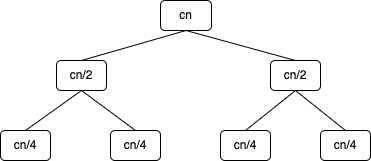
\includegraphics[width=.9\linewidth]{assets/desarrollo_concurrencia.png}
\end{center}

En el nivel 1 se realizan cn operaciones, en el segundo \(cn/2 * 2 = cn\) operaciones, en el tercero \(cn/4 * 4 = cn\) operaciones y en un nivel genérico \(j\) se realizan \(cn/2^{j-1} * 2^{j-1} = cn\) operaciones.

Luego es necesario calcular la cantidad de niveles que tendrá nuestro algoritmo. Para ello utilizaremos el caso base en el cual hay problemas con solo 2 elementos, por lo tanto podemos plantear que en dicho nivel \(k\) hay \(2^k\) subproblemas que equivale a la mitad de los elementos de nuestro problema dado que utilizamos un caso base con 2 elementos. Consecuentemente, \(2^k = n/2 \Rightarrow k * log_2 2 = log_2 (n/2) \Rightarrow k = log_2 n - 1\).

Finalmente, al multiplicar la cantidad de operaciones a realizar en cada nivel por la cantidad total de niveles obtenemos que la complejidad temporal es \(O(cn * (log_2 n - 1)) = O(n * log_2 n)\)

\subsubsection{Complejidad espacial}
\label{sec:org8e33d4c}

La única estructura adicional al arreglo provisto como entrada del algoritmo es un diccionario/lista que contabilice la cantidad de inversiones de cada elemento. Como en el peor de los casos todos los elementos cuentan con inversiones, se considera que el arreglo puede tener hasta \(n\) elementos. La división de listas en mitades depende de la implementación del algoritmo.

En conclusión, el algoritmo tiene una complejidad espacial de \(E(n) = O(n)\)

\subsection{Ejemplo de funcionamiento}
\label{sec:org169ce63}

Tomaremos como caso el ejemplo dado por la cátedra, pero realizaremos una modificación para que sean 8 jugadores en lugar de 6. De manera que la lista de entrada estará dada por las tuplas (id,ranking): A,3 | B,4 | C,2 | D,8 | E,6 | F,5 | H,7 | G,1

A continuación se muestran los subproblemas a resolver. A fin de mostrar cómo se construye el diccionario de superados, se decidió seguir un orden cronológico de resolución. Dado que se comienza procesando la primer mitad de la lista, comenzaremos resolviendo la rama izquierda del árbol; el órden nos lleva al subproblema con los primeros dos elementos, y comenzaremos resolviendo el árbol desde allí.

\begin{center}
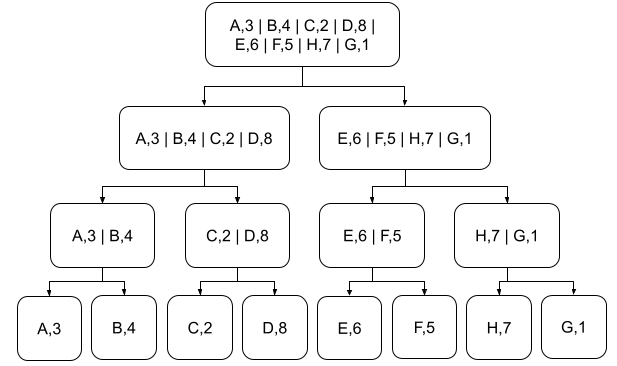
\includegraphics[width=.9\linewidth]{assets/subproblemas.png}
\end{center}

\begin{minted}[bgcolor=bg]{text}
lista = A,3 | B,4

lista_inf = rivales_superados_rec(A,3; superados) = A,3    # caso base
lista_inf = rivales_superados_rec(B,4; superados) = B,4    # caso base

# no hay inversiones
lista_final = unir_y_contar(A,3 | B,4; superados) = A,3 | B,4

superados = {  }
\end{minted}

\noindent\rule{\textwidth}{0.5pt}

\begin{minted}[bgcolor=bg]{text}
lista = C,2 | D,8

lista_inf = rivales_superados_rec(C,2; superados) = C,2    # caso base
lista_sup = rivales_superados_rec(D,8; superados) = D,8  # caso base

# no hay inversiones
lista_final = unir_y_contar(C,2; D,8; superados) = C,4 | D,8

superados = { }
\end{minted}

\noindent\rule{\textwidth}{0.5pt}


\begin{minted}[bgcolor=bg]{text}
lista = A,3 | B,4 | C,2 | D,8

lista_inf = rivales_superados_rec(A,3 | B,4; superados) = A,3 | B,4
lista_sup = rivales_superados_rec(C,2 | D,8; superados) = C,2 | D,8

# inversiones (A, C), (B, C)
lista_final = unir_y_contar(A,3 | B,4; C,2 | D,8; superados) = C,2 | A,3 | B,4 | D,8

superados = { A: 1, B: 1}
\end{minted}

\noindent\rule{\textwidth}{0.5pt}

Comenzamos la resolución con la otra rama del árbol:

\begin{minted}[bgcolor=bg]{text}
lista = E,6 | F,5

lista_inf = rivales_superados_rec(E,6; superados) = E,6   # caso base
lista_sup = rivales_superados_rec(F,5; superados) = F,5  # caso base

# inversion (E, F)
lista_final = unir_y_contar(E,6; F,5; superados) = F,5 | E,6

superados = { A: 1, B: 1, E: 1}
\end{minted}

\noindent\rule{\textwidth}{0.5pt}
\begin{minted}[bgcolor=bg]{text}
lista = H,7 | G,1

lista_inf = rivales_superados_rec(H,7; superados) = H,7      # caso base
lista_sup = rivales_superados_rec(G,1; superados) = G,1   # caso base

# detectamos que el ranking de G es menor al de H, por lo que están invertidos
lista_final = unir_y_contar(H,7; G,1; superados) = G,1 | H,7

superados = { A: 1, B: 1, E: 1, H: 1 }
\end{minted}

\noindent\rule{\textwidth}{0.5pt}

\begin{minted}[bgcolor=bg]{text}
lista = E,6 | F,5 | H,7 | G,1

lista_inf = rivales_superados_rec(E,6 | F,5; superados) = F,5 | E,6
lista_sup = rivales_superados_rec(H,7 | G,1; superados) = G,1 | H,7

# inversiones (F, G) y (E, G)
lista_final = unir_y_contar(F,5 | E,6; G,1 | H,7; superados) = G,1 | F,5 | E,6 | H,7

superados = { A: 1, B: 1, E: 2, F: 1, H: 1 }
\end{minted}

\noindent\rule{\textwidth}{0.5pt}

Finalmente unimos los subproblemas en el original:

\begin{minted}[bgcolor=bg]{text}
lista = A,3 | B,4 | C,2 | D,8 | E,6 | F,5 | H,7 | G,1

lista_inf = rivales_superados_rec(A,3 | B,4 | C,2 | D,8; superados) = C,2 | A,3 | B,4 | D,8
lista_sup = rivales_superados_rec(E,6 | F,5 | H,7 | G,1, superados) = G,1 | F,5 | E,6 | H,7

# inversiones (A, G), (B, G), (C, G), (D, G)
lista_final = unir_y_contar(lista_inf; lista_sup; superados)

superados = { A: 2, B: 2, C: 1, D: 1, E: 2, F: 1, H: 1} # resultado final
\end{minted}

\noindent\rule{\textwidth}{0.5pt}

\newpage

\section{Parte 2: Ciclos negativos}
\label{sec:org2a9e959}

En esta segunda parte del trabajo practico, se nos presenta el problema de
analizar un grafo dirigido ponderado con valores enteros y verificar si tiene,
por lo menos, un ciclo negativo. En el caso de tenerlo, debemos mostrar en
pantalla los nodos que contienen a dicho ciclo. Además, se nos pide que la
solución presentada utilice programación dinámica.

\subsection{Solución con Bellman-Ford}
\label{sec:orge47cb61}
Para resolver el problema enunciado podemos utilizar el algoritmo Bellman-Ford
para calcular el camino mínimo en un grafo ponderado con aristas negativas a
partir de un nodo de origen. Lógicamente, no podría encontrarse un camino mínimo
distinto a (menos infinito) si es que hay ciclos negativos. Esto es porque
caeríamos en un punto donde resulta conveniente recorrer dicho ciclo
infinitamente ya que cada vez se reduce más la longitud del camino mínimo. Vamos
a ver que esto puede ser utilizado para encontrar ciclos negativos.


\hfill

Primero, veamos como calcular el camino mínimo:

\subsubsection{Algoritmo}
\label{sec:org95ceee9}

Primero, se inicializa la distancia del nodo de origen \(n_s\) hasta todos los
vértices como infinito y la distancia al nodo \(n_s\) como cero. Luego por cada
arista se verifica si la distancia guardada para llegar al vértice de origen de
la arista sumado al peso de la arista es menor a la guardada para llegar al
vértice destino de la arista. Esto se repite \(N – 1\) veces con \(N\) el número de
nodos del grafo. De esta manera, en cada iteración \(i\), el algoritmo encuentra el
camino mínimo de longitud máxima \(i\). Es por esto que el ciclo se repite \(N – 1\)
veces, porque el camino mínimo sin ciclos podría ser de esa longitud. Es en este
punto donde el algoritmo nos es de utilidad. Podemos aplicar el mismo
procedimiento una vez, es decir viendo si se puede encontrar un camino mínimo de
longitud \(N\) que sea menor al encontrado de longitud \(N – 1\). Si esto sucede,
implica que estamos agregando una arista negativa formando un ciclo negativo. Es
decir, identificamos el ciclo negativo que se nos pide en el enunciado.

\hfill

El algoritmo de Bellman-Ford termina ahí, en el caso de encontrar un ciclo
negativo devuelve error y en caso contrario devuelve el camino mínimo o una
estructura para reconstruirlo. En nuestro caso, necesitamos adaptar el algoritmo
para que devuelva un ciclo negativo si es que hay o nada en caso de no haber.
Entonces, lo que podemos hacer es una vez que sabemos que hay un ciclo negativo,
iterar una vez mas y reconstruir el ciclo negativo.

\pagebreak

\begin{enumerate}
\item Pseudo-codigo
\label{sec:org68874d9}

\begin{minted}[bgcolor=bg]{text}
funcion Bellman_Ford(Grafo grafo, Nodo origen)
    siendo distancias un diccionario
    siendo predecesores un diccionario

    por cada vertice v del grafo:
        distancias[v] = infinito

    distancias[origen] = 0
    padres[origen] = None

    por cada vertice:
        por cada arista de origen v y destino w y peso:
            si distancias[v] + peso < distancias[w]:
                predecesores[w] = v
                distancias[w] = distintas[v] + peso

    por cada arista de origen v y destino w y peso:
        si distancias[v] + peso < distancias[w]:
            tirar error "Hay un ciclo negativo"
\end{minted}
\end{enumerate}

\subsubsection{Sub-estructura optima}
\label{sec:org6824cee}

Para calcular las distancias mínimas de un nodo hacia otro se utiliza la
distancia mínima calculado anteriormente para su predecesor mas el peso de
llegar a el. Entonces la subestructura seria los caminos mínimos de todos los
nodos predecesores al nodo final.

\subsubsection{Complejidad}
\label{sec:org89e422f}

Podemos analizar la complejidad temporal a partir del pseudo-codigo. Primero,
tenemos un ciclo donde inicializamos las distancias de cada vértice al origen
como infinito. Es decir \texttt{O(V)}, donde V es la cantidad de vértices. Luego, por
cada vértice sin contar el origen recorremos todas las aristas que resulta
\texttt{O(E)}. Es decir que el ciclo entero tiene una complejidad de \texttt{O(V * E)}.
Finalmente, encontrar el ciclo negativo y devolverlo tiene una complejidad de
\texttt{O(E)} porque se recorren todas las aristas una vez más.  Entonces, la
complejidad final del algoritmo es de \texttt{O(V * E)}.

Y la complejidad espacial es \texttt{O(V)}. porque almacenamos dos diccionarios para
las distancias y los predecesores que son de maximo \texttt{V}.

\subsubsection{Relación de Recurrencia}
\label{sec:org341e834}

Sea \(n_s\) en nodo de inicio, \(T\) el nodo final, \(N_i\) un nodo y \(predecesores[N_i]\) es el
conjunto de los nodos adyacentes a \(N_i\), sabemos que para llegar desde el nodo \(n_s\)
al nodo \(N_i\) en una cantidad de pasos \(j\) debemos haber llegado a alguno de sus
predecesores en \(j-1\) pasos. Entonces, siendo la longitud la cantidad de nodos que
se recorren hasta llegar al nodo \(N_i\), se deduce de lo planteado que el camino
mínimo hasta el nodo \(N_i\) dada una longitud máxima \(L\) es el mínimo de los caminos
hacia sus predecesores mas la longitud de llegar del predecesor a \(N_i\). Por lo
tanto, nuestra ecuación de recurrencia resulta:

Definiendo:
\begin{itemize}
\item \(n_s\): nodo origen o \emph{source node}
\item \(n_i\): otro nodo distinto al origen
\item \(j\): longitud máxima para llegar de \(n_s\) a \(n_i\)
\item \(minPath(n_i, j)\): función recursiva para llegar al camino mínimo de \(s\) a \(n_i\)
\item \(n_x\): predecesores a \(n_i\)
\item \(k\): cantidad de predecesores a \(n_i\)
\item \(w(n_x,n_i)\): peso de la arista \(n_x\) y \(n_i\)
\end{itemize}

$$minPath(n_s, j) = 0$$
$$minPath(n_i, 0) = +\infty\ \text{con}\ n_i \neq S$$
$$
minPath(n_i, j) = min \left\{\begin{array}{lcc}
                        minPath(n_i, j-1) \\
                        min\ \left\{\begin{array}{lcc}
                               minPath(n_x_1, j-1) + w(n_x_1,n_i) \\
                               minPath(n_x_2, j-1) + w(n_x_2,n_i) \\
                               ... \\
                               minPath(n_x_k, j-1) + w(n_x_k,n_i)
                             \end{array}\right\}
                      \end{array}\right\}
$$

\subsection{Detalles de implementación}
\label{sec:orgde612e8}

El algoritmo fue implementado en Python y no tiene dependencias aparte de tener
instalado cualquier versión de \texttt{python3}.

\subsubsection{Ejecución del programa}
\label{sec:org9b25fe7}

El programa contiene un \texttt{shebang} para ser ejecutado en una terminal de la
siguiente forma:

\begin{minted}[bgcolor=bg]{bash}
./src/parte_2.py <filename>
\end{minted}

El comprimido entregado incluye un archivo ejemplo en \texttt{assets/grafo.txt} con grafos ejemplos,
por ejemplo:

\begin{minted}[bgcolor=bg]{text}
B
D,A,-2
B,A,3
D,C,2
C,D,-1
B,E,2
E,D,-2
A,E,3
\end{minted}

\begin{minted}[bgcolor=bg]{bash}
./src/parte_2.py ./assets/grafo.txt
\end{minted}

\begin{minted}[bgcolor=bg]{text}
Existen al menos un ciclo negativo en el grafo. A,E,D → costo: -1
\end{minted}

\subsubsection{Estructuras de datos}
\label{sec:org60e6d2f}

Para la representación del grafo decidimos manteneral simple:
\begin{itemize}
\item Un lista de aristas para almacenar las aristas tal cual como estan en el archivo.
\item Un set de vértices para mantener un registro de los vértices ingresados en
cada arista.
\end{itemize}

\pagebreak

\subsubsection{Implementación de Bellman-Ford en Python}
\label{sec:org0307ca9}

Al igual que el pseudo-codigo, podemos describir la implementación de la
siguiente manera:

\begin{enumerate}
\item Iniciamos:
\begin{itemize}
\item un diccionario de distancias con clave \texttt{vertice} y valor infinito.
\item un diccionario de predecesores donde la clave \texttt{origen} se inicializa en \texttt{None}
\item la distancia de clave \texttt{origen} se cambia a \texttt{0}.
\end{itemize}
\item Iterar por la cantidad de vértices del grafo:
\begin{itemize}
\item por cada arista, si la distancia guardada para llegar al origen de la
arista mas el peso de moverse al nodo destino de la arista es menor a la
distancia guardada para llegar al nodo destino de la arista, reemplazar la
distancia guardada del nodo destino.
\item ademas, verificamos si no hubo un cambio en la iteración de aristas, si
este es el caso, podemos confirmar que no existe ningún ciclo negativo
por lo que devolvemos.
\end{itemize}
\item Verificar que no haya ciclos negativos
\begin{itemize}
\item por cada arista, si se sigue cumpliendo la condición del punto anterior,
entonces hay un ciclo negativo
\item si hay un ciclo negativo:
\begin{itemize}
\item reconstruir los nodos predecesores hasta llegar al nodo que se detecto
y sumar los pesos de sus aristas.
\item devolver el ciclo negativo y su peso
\end{itemize}
\end{itemize}
\end{enumerate}

\subsubsection{Calcular ciclo negativo}
\label{sec:orga7901d7}

A partir del algoritmo de Bellman-Ford agregamos código cuando se detecta el
ciclo negativo que agrega el nodo que se detecto termina el ciclo negativo y se
reconstruye los nodos predecesores iterando hasta volver al nodo original
mientras que se suman todos sus pesos en la variable \texttt{peso\_ciclo}.

Luego devolvemos al \texttt{ciclo} reconstruido invertido y el \texttt{peso\_ciclo} calculado.

\subsubsection{Complejidad de la implementación}
\label{sec:org95950ba}

Con la simple estructura que decidimos usar, el codigo y el pseudo-codigo tiene
pocas diferencias, y la complejidad temporal termina siendo la misma \(O(V * E)\).

En el código de Python tenemos las siguiente operaciones:
\begin{itemize}
\item Inicializar las distancias en infinito que lo hacemos con un simple \texttt{for}
sobre \texttt{grafo.vertices} por lo que la complejidad computacional es \texttt{O(V)}.
\item Luego hacemos un \texttt{for} anidado entre \texttt{grafo.vertices} (un \emph{set} de python) y
\texttt{grafo.aristas} (un \emph{lista} de python), y como decidimos tener estructura
simple (cuando creamos el grafo almacenamos los vértices y las aristas como
vienen), la complejidad termina siendo la multiplicación de los dos ciclos es
decir \texttt{O(V * E)} ya que en Python tanto iterar sobre listas o sobre sets es
\texttt{O(n)}.
\item Ademas, en la búsqueda de ciclos negativos hacemos uso de \texttt{grafo.peso()}, que
por la estructura que tenemos es \texttt{O(E)} por lo que como ademas iteramos sobre
todas las aristas esa parte queda \texttt{O(V * E)}.
\end{itemize}

Y la complejidad espacial es \texttt{O(V)} porque solo guardamos dos diccionarios de
largo \texttt{V}, uno con las distancias y otro con los predecesores y en caso de
encontrar un ciclo negativo es como mucho de largo \texttt{V}, lo que en el peor de los
casos es \texttt{O(3*V)} que es \texttt{O(V)}.

\newpage

\section{Parte 3: Un poco de teoría}
\label{sec:org0792ea6}

\subsection{División y Conquista}
\label{sec:org84303ed}

La división y conquista es una técnica algorítmica que consiste en 3 elementos
claves. El primero es, dividir el problema en N subproblemas menores pero que se
puedan resolver igual. Luego, resolver estos problemas de manera recursiva
planteando un caso base, es decir un caso donde el problema se resuelva de forma
trivial y no haga falta dividirlo. Finalmente, se combina la solución hallada de
todos los subproblemas para formar la solución general.

Entonces, es evidente que para que un problema se pueda resolver por división y
conquista debe tener subestructura optima. La complejidad temporal utilizando
esta estrategia se calcula una vez obtenida la relación de recurrencia del
problema. Para ello, se puede, o bien desarrollar la relación de recurrencia
matemáticamente utilizando el costo del caso base o, utilizar el Teorema
Maestro. Este ultimo teorema, no necesariamente resuelve todos los problemas de
división y conquista pero por lo general es una herramienta muy útil.

\subsection{Programacion Dinamica}
\label{sec:org70be68c}

La programación dinámica resuelve problemas de índole de optimización. Para 
ello, el problema tiene que tener dos características: Subestructura óptima y 
Subproblemas superpuestos. La primera, implica que la resolución de un 
problema global contiene resoluciones óptimas de sus subproblemas. La segunda, 
refiere a la aparición de subproblemas previamente calculados. Esta última 
propiedad es la que se aprovecha junto a técnicas de programación como la 
memorización para reducir la complejidad del algoritmo. Al guardarse los 
resultados óptimos de los subproblemas, se evita tener que volver a calcularlos. 
La complejidad de este tipo de algoritmo se calcula con una relación de 
recurrencia la cual tiene en cuenta un caso base y la resolución de un problema 
N en relacion a un problema N-1. En forma iterativa, entonces, se procede a 
calcular los subproblemas más chicos cuyos resultados serán utilizados 
para los siguientes.

\subsection{Comparación de estrategias}
\label{sec:org791b5e3}

No existe una mejor estrategia, algunos problemas directamente no se pueden
plantear usando una de las tres estrategias vistas, por lo que categorizar una
como la mejor no tiene sentido.

En el caso de poder resolverse con npas de una, se elige la estrategia 
que resuelva el problema, o con mejor complejidad temporal, o menor complejidad espacial,
como se ejemplifica en el para el siguiente problema:

\subsection{El problema}
\label{sec:org7d9bce7}

Se trabaja sobre una matriz. El ejercicio no da mucha información acerca de la
complejidad espacial, por lo que tenemos dar supuestos:

El Algoritmo Greedy realiza \(N^3\) operaciones sobre la matriz. En primero lugar,
podríamos suponer que la complejidad espacial es \(O(K)\), con \(K\) una constante. 
En el caso de Programación Dinámica que divide el problema en \(n^2\) sub-problemas,
podríamos decir que la complejidad espacial de este ultimo es \(O(K * n^2)\) por lo 
que siempre se cumpliría que la complejidad espacial de Programación Dinámica es
mayor a la del Algoritmo Greedy.

El de Programación Dinámica realiza \(N^2\) operaciones sobre la matriz, por lo que
la \emph{complejidad temporal} del Algoritmo Greedy es menor Programación Dinámica.

Frente a dos algoritmos que resuelven el mismo problema, siempre se deberia
elegir aquel que tenga menor complejidad temporal y espacial. En caso de tener
igual complejidad espacial, se elige el de menor complejidad temporal y
viceversa.

El problema surgue cuando uno tiene una complejidad mayor que la otra,
en ese caso debe tenerse en cuenta las características y condiciones 
del sistema donde se va a ejecutar.

\subsubsection{¿Porque eligiria el Algoritmo Greedy?}
\label{sec:org383e928}
Si yo tengo poca memoria (como el caso de sistema embedidos), yo tal vez ni
siquiera tendria la posibilidad de poder ejecutar el algoritmo con Programación
Dinamica porque no tengo suficiente memoria para procesarlo.

\subsubsection{¿Porque eligiria el de Programación Dinámica?}
\label{sec:orgeaf1eb4}
En computadoras modernas, la mayoría de los sistemas vienen con bastante memoria
(>8GB) entonces podría despreciar el hecho de que necesito mas memoria para
procesar el algoritmo en orden de ganar en tiempo de ejecución.

\subsubsection{Conclusión}
\label{sec:org4769eb3}
No hay un algoritmo perfecto para todos los casos, solo hay algoritmos optimos
para un problema. Elegir entre un algoritmo que tiene complejidad espacial
\(O(n^2)\) y complejidad espacial \(O(n^2)\), y otro algoritmo de complejidad espacial
\(O(1)\) y complejidad temporal \(O(n^3)\), dependiendo de las condiciones donde se
ejecuta, el algoritmo eligiria uno sobre otro, pero la realidad es que, a menos
que este trabajando en sistemas embebidos (o algun sistema especifico con muy
poca memoria), es mas probable que priorice la complejidad temporal que la
espacial.
\end{document}
